\documentclass{standalone}
\usepackage{tikz}
\usetikzlibrary{patterns, positioning}
\usepackage[sfdefault]{ClearSans} %% option 'sfdefault' activates Clear Sans as the default text font
\usepackage[T1]{fontenc}

\begin{document}
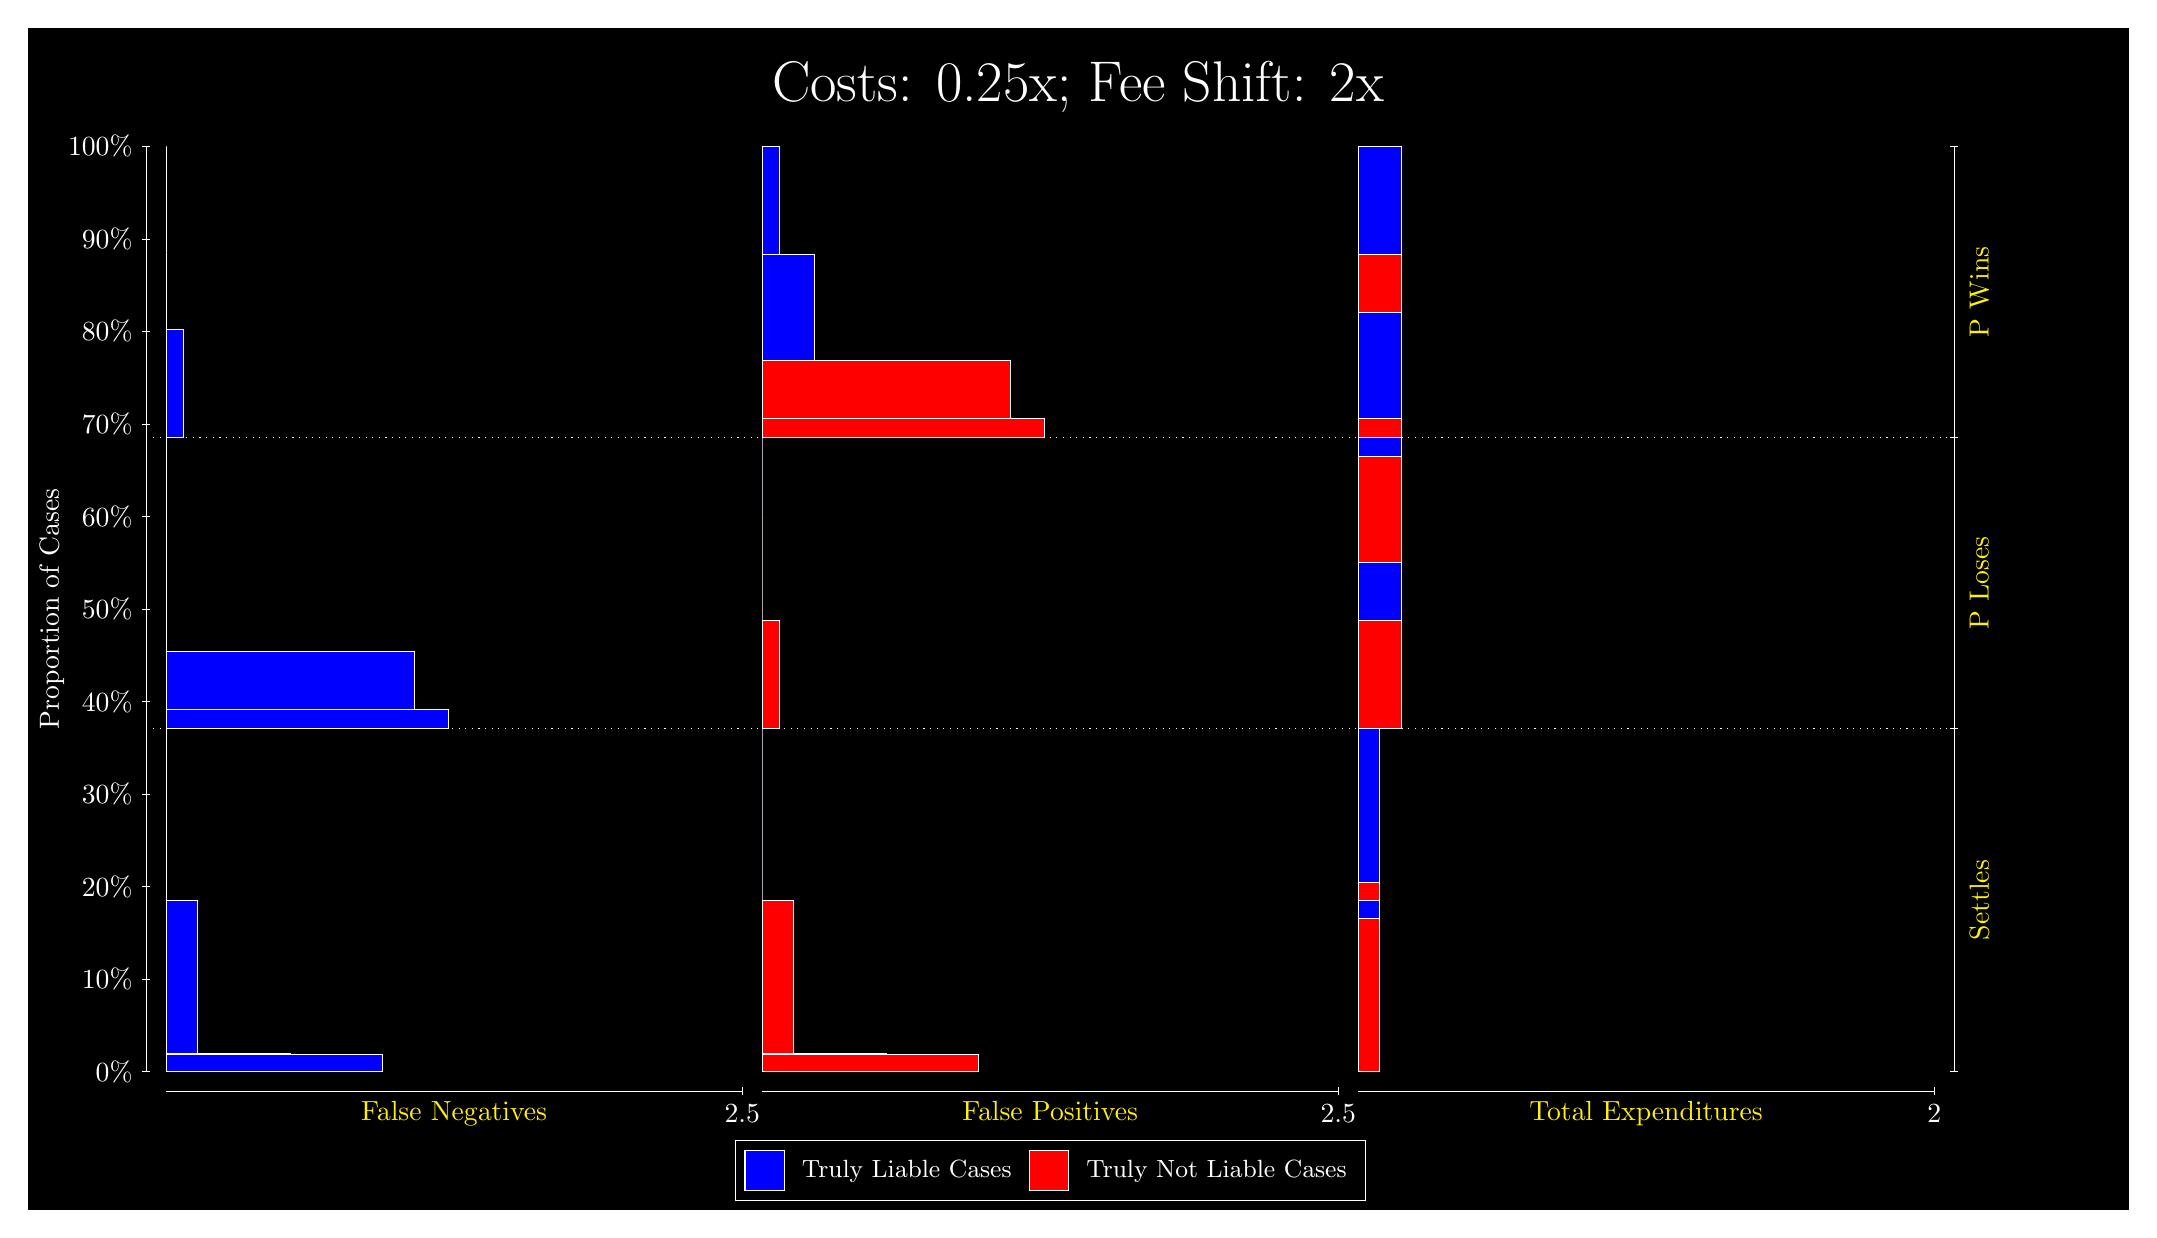
\begin{tikzpicture}
\draw[fill=black] (0,0) rectangle (26.667,15);
\draw[text=white] (0,13.5) rectangle (26.667,15) node[midway] {\huge Costs: 0.25x; Fee Shift: 2x};
\draw[white, very thin] (1.5,1.75) -- (1.5,13.5);
\node[rotate=90, text=white, anchor=center] at (0.3, 7.625) {Proportion of Cases};
\draw[white, very thin] (1.45,1.75) -- (1.55,1.75);
\node[text=white, anchor=east] at (1.45, 1.75) {0\%};
\draw[white, very thin] (1.45,2.925) -- (1.55,2.925);
\node[text=white, anchor=east] at (1.45, 2.925) {10\%};
\draw[white, very thin] (1.45,4.1) -- (1.55,4.1);
\node[text=white, anchor=east] at (1.45, 4.1) {20\%};
\draw[white, very thin] (1.45,5.275) -- (1.55,5.275);
\node[text=white, anchor=east] at (1.45, 5.275) {30\%};
\draw[white, very thin] (1.45,6.45) -- (1.55,6.45);
\node[text=white, anchor=east] at (1.45, 6.45) {40\%};
\draw[white, very thin] (1.45,7.625) -- (1.55,7.625);
\node[text=white, anchor=east] at (1.45, 7.625) {50\%};
\draw[white, very thin] (1.45,8.8) -- (1.55,8.8);
\node[text=white, anchor=east] at (1.45, 8.8) {60\%};
\draw[white, very thin] (1.45,9.975) -- (1.55,9.975);
\node[text=white, anchor=east] at (1.45, 9.975) {70\%};
\draw[white, very thin] (1.45,11.15) -- (1.55,11.15);
\node[text=white, anchor=east] at (1.45, 11.15) {80\%};
\draw[white, very thin] (1.45,12.325) -- (1.55,12.325);
\node[text=white, anchor=east] at (1.45, 12.325) {90\%};
\draw[white, very thin] (1.45,13.5) -- (1.55,13.5);
\node[text=white, anchor=east] at (1.45, 13.5) {100\%};

\draw[white, very thin] (24.457,1.75) -- (24.457,13.5);
\draw[white, very thin] (24.407,1.75) -- (24.507,1.75);
\node[anchor=west] at (24.407, 1.75) {};
\draw[white, very thin] (24.407,6.1067) -- (24.507,6.1067);
\node[anchor=west] at (24.407, 6.1067) {};
\draw[white, very thin] (24.407,9.8034) -- (24.507,9.8034);
\node[anchor=west] at (24.407, 9.8034) {};
\draw[white, very thin] (24.407,13.5) -- (24.507,13.5);
\node[anchor=west] at (24.407, 13.5) {};

\draw[white, very thin, fill=blue] (1.75,1.75) rectangle (4.4946,1.9721);
\draw[white, very thin, fill=blue] (1.75,1.9721) rectangle (3.3236,1.98);
\draw[white, very thin, fill=blue] (1.75,1.98) rectangle (2.1525,3.9283);
\draw[white, very thin, fill=red] (1.75,3.9283) rectangle (1.75,6.1067);
\draw[white, very thin, fill=blue] (1.75,6.1067) rectangle (5.3362,6.3443);
\draw[white, very thin, fill=blue] (1.75,6.3443) rectangle (4.8971,7.0866);
\draw[white, very thin, fill=red] (1.75,7.0866) rectangle (1.75,9.8034);
\draw[white, very thin, fill=blue] (1.75,9.8034) rectangle (1.9696,11.175);
\draw[white, very thin, fill=red] (1.75,11.175) rectangle (1.75,12.154);
\draw[white, very thin, fill=blue] (1.75,12.154) rectangle (1.75,13.5);
\draw[white, very thin, fill=red] (9.3189,1.75) rectangle (12.063,1.9721);
\draw[white, very thin, fill=red] (9.3189,1.9721) rectangle (10.892,1.98);
\draw[white, very thin, fill=red] (9.3189,1.98) rectangle (9.7214,3.9284);
\draw[white, very thin, fill=blue] (9.3189,3.9284) rectangle (9.3189,6.1067);
\draw[white, very thin, fill=red] (9.3189,6.1067) rectangle (9.5384,7.4779);
\draw[white, very thin, fill=red] (9.3189,7.4779) rectangle (9.3189,8.8235);
\draw[white, very thin, fill=blue] (9.3189,8.8235) rectangle (9.3189,9.8034);
\draw[white, very thin, fill=red] (9.3189,9.8034) rectangle (12.905,10.041);
\draw[white, very thin, fill=red] (9.3189,10.041) rectangle (12.466,10.783);
\draw[white, very thin, fill=blue] (9.3189,10.783) rectangle (9.9776,12.129);
\draw[white, very thin, fill=blue] (9.3189,12.129) rectangle (9.5384,13.5);
\draw[white, very thin, fill=red] (16.888,1.75) rectangle (17.162,3.6984);
\draw[white, very thin, fill=blue] (16.888,3.6984) rectangle (17.162,3.9205);
\draw[white, very thin, fill=red] (16.888,3.9205) rectangle (17.162,4.1505);
\draw[white, very thin, fill=blue] (16.888,4.1505) rectangle (17.162,6.1067);
\draw[white, very thin, fill=red] (16.888,6.1067) rectangle (17.437,7.4779);
\draw[white, very thin, fill=blue] (16.888,7.4779) rectangle (17.437,8.2202);
\draw[white, very thin, fill=red] (16.888,8.2202) rectangle (17.437,9.5658);
\draw[white, very thin, fill=blue] (16.888,9.5658) rectangle (17.437,9.8034);
\draw[white, very thin, fill=red] (16.888,9.8034) rectangle (17.437,10.041);
\draw[white, very thin, fill=blue] (16.888,10.041) rectangle (17.437,11.387);
\draw[white, very thin, fill=red] (16.888,11.387) rectangle (17.437,12.129);
\draw[white, very thin, fill=blue] (16.888,12.129) rectangle (17.437,13.5);
\draw[white, dotted] (1.5,6.1067) -- (24.457,6.1067);
\draw[white, dotted] (1.5,9.8034) -- (24.457,9.8034);
\draw[white, very thin] (1.75,1.5) -- (9.0689,1.5);
\node[text=yellow, anchor=north] at (5.4094, 1.5) {False Negatives};
\draw[white, very thin] (9.0689,1.45) -- (9.0689,1.55);
\node[text=white, anchor=north] at (9.0689, 1.45) {2.5};

\draw[white, very thin] (9.3189,1.5) -- (16.638,1.5);
\node[text=yellow, anchor=north] at (12.978, 1.5) {False Positives};
\draw[white, very thin] (16.638,1.45) -- (16.638,1.55);
\node[text=white, anchor=north] at (16.638, 1.45) {2.5};

\draw[white, very thin] (16.888,1.5) -- (24.207,1.5);
\node[text=yellow, anchor=north] at (20.547, 1.5) {Total Expenditures};
\draw[white, very thin] (24.207,1.45) -- (24.207,1.55);
\node[text=white, anchor=north] at (24.207, 1.45) {2};

\node[text=yellow, centered, rotate=90] at (24.777, 3.9284) {Settles};
\node[text=yellow, centered, rotate=90] at (24.777, 7.955) {P Loses};
\node[text=yellow, centered, rotate=90] at (24.777, 11.652) {P Wins};

\draw (12.978300999999998,1.5) node[draw=none] (baseCoordinate) {};
\begin{scope}[align=center]
        \matrix[scale=0.5, draw=white, below=0.5cm of baseCoordinate, nodes={draw}, column sep=0.1cm]{
            \node[rectangle, draw, minimum width=0.5cm, minimum height=0.5cm, fill=blue] {}; &
            \node[draw=none, font=\small, text=white] (B) {Truly Liable Cases}; &
            \node[rectangle, draw, minimum width=0.5cm, minimum height=0.5cm, fill=red] {}; &
            \node[draw=none, font=\small, text=white] (B) {Truly Not Liable Cases}; \\
            };
\end{scope}

\end{tikzpicture}
\end{document}